\chapter{Higher algebraic structures}
\label{part:higherAlgebraicStructures}

In this third part, we derive some higher algebraic consequences of the results obtained in \cref{part:diagonalsPermutahedra}.
We first prove in \cref{subsec:top-operadic-structures} that there are exactly two topological operad structures on the family of operahedra (\resp multiplihedra) which are compatible with the generalized Tamari order, and thus two geometric universal tensor products of (non-symmetric non-unital) homotopy operads (\resp $\Ainf$-morphisms).
Then, we show that these topological operad structures are isomorphic (\cref{subsec:iso-top-operads}).
However, these isomorphisms do not commute with the diagonal maps (\cref{ex:iso-not-Hopf,ex:iso-not-Hopf-2}).
Finally, we show that contrary to the case of permutahedra, the faces of the $\LA$ and $\SU$ diagonals of the operahedra (\resp multiplihedra) are in general not in bijection (\cref{subsec:tensor-products}).
However, from a homotopical point of view, the two tensor products of homotopy operads (\resp $\Ainf$-morphisms) that they define are $\infty$-isomorphic (\cref{thm:infinity-iso,thm:infinity-iso-2}). 

%%%%%%%%%%%%%%%%%%%%%%%%%%%%%%%%%%%%%%

\section{Higher tensor products}

%%%%%%%%%%%%%%%

\subsection{Topological operadic structures}
\label{subsec:top-operadic-structures}

The permutahedra are part of a more general family of polytopes called Loday realizations of the \emph{operahedra}~\cite[Def.~2.9]{LaplanteAnfossi}, which encodes the notion of homotopy operad~\cite[Def.~4.11]{LaplanteAnfossi} (we consider here only \emph{non-symmetric non-unital} homotopy operads).
Let $\PT_n$ be the set of planar trees with $n$ internal edges, which are labelled by $[n]$ using the infix order.
For every planar tree $t$, there is a corresponding operahedron $P_t$ whose codimension~$k$ faces are in bijection with nestings of $t$ with $k$ non-trivial nests.

\begin{definition}[{\cite[Def.~2.1 \& 2.22]{LaplanteAnfossi}}]\label{def:nesting}
	A \defn{nest} of $t \in \PT_n$ is a subset of internal edges which induce a subtree, and a \defn{nesting} of $t$ is a family of nests which are either included in one another, or disjoint.
	See \cref{fig:nestings}.
\end{definition}

\begin{figure}[h!]
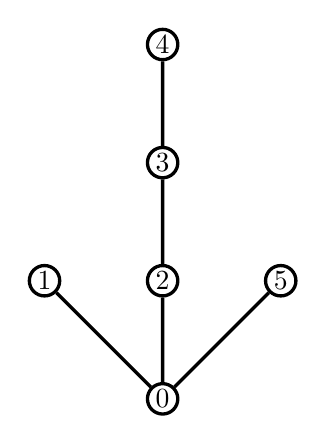
\begin{tikzpicture}[yscale=-1, every node/.style={draw, very thick, circle, inner sep=1pt}, edge from parent path={[very thick, draw] (\tikzparentnode) -- (\tikzchildnode)}]
]
\node(0) {0}
	child{node(1){1}}
	child{node(2){2}
		child{node(3){3}
		child{node(4){4}}
		}}
	child{node(5){5}};
% \begin{pgfonlayer}{bg}    % select the background layer
\hedge[blue, very thick]{0,2,1}{0.3cm}
\hedge[violet, very thick]{0,2,3,1}{0.4cm}
\hedge[red, very thick]{0,5,4,1}{0.5cm}
%\end{pgfonlayer}
\end{tikzpicture}
\qquad
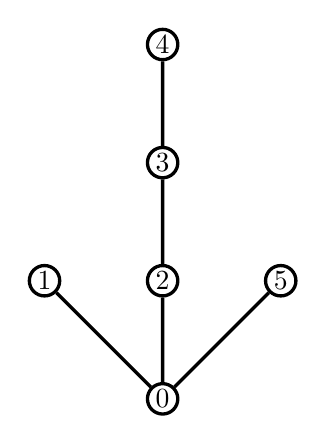
\begin{tikzpicture}[yscale=-1, every node/.style={draw, very thick, circle, inner sep=1pt}, edge from parent path={[very thick, draw] (\tikzparentnode) -- (\tikzchildnode)}]
	]
	\node(0) {0}
		child{node(1){1}}
		child{node(2){2}
			child{node(3){3}
			child{node(4){4}}
			}}
		child{node(5){5}};
	% \begin{pgfonlayer}{bg}    % select the background layer
	\hedge[blue, very thick]{2,3}{0.3cm}
	\hedge[blue, very thick]{0,5}{0.3cm}
	\hedge[violet, very thick]{0,5,3}{0.4cm}
	\hedge[red, very thick]{0,5,4,1}{0.5cm}
	%\end{pgfonlayer}
\end{tikzpicture}
\caption{Two nestings of a tree with $5$ internal edges. These nestings, \cref{def:nesting}, are also $2$-colored, \cref{def:2-Colored Nesting}.}
\label{fig:nestings}
\end{figure}

Since the operahedra are generalized permutahedra~\cite[Coro.~2.16]{LaplanteAnfossi}, a choice of diagonal for the permutahedra induces a choice of diagonal for every operahedron~\cite[Coro.~1.31]{LaplanteAnfossi}.
Every face of an operahedron is isomorphic to a product of lower-dimensional operahedra, via an isomorphism~$\Theta$ which generalizes the one from \cref{subsec:operadicProperty}, see Point (5) of~\cite[Prop.~2.3]{LaplanteAnfossi}.

\begin{definition}
An \emph{operadic diagonal} for the operahedra is a choice of diagonal $\triangle_t$ for each Loday operahedron~$P_t$, such that $\triangle \eqdef \{\triangle_t\}$ commutes with the map $\Theta$, \ie it satisfies~\cite[Prop.~4.14]{LaplanteAnfossi}.
\end{definition}

An operadic diagonal gives rise to topological operad structure on the set of Loday operahedra \cite[Thm 4.18]{LaplanteAnfossi}, and via the functor of cellular chains, to a universal tensor product of homotopy operads \cite[Prop. 4.27]{LaplanteAnfossi}. 
Here, by \defn{universal}, we mean a formula that applies uniformly to \emph{any} pair of homotopy operads. 
Since such an operad structure and tensor product are induced by a geometric diagonal, we shall call them \defn{geometric}.

\begin{theorem}
\label{thm:operahedra}
There are exactly 
\begin{enumerate}
\item two geometric operadic diagonals of the Loday operahedra, the $\LA$ and $\SU$ diagonals,
\item two geometric colored topological cellular operad structures on the Loday operahedra,
\item two geometric universal tensor products of homotopy operads,
\end{enumerate}
which agree with the generalized Tamari order on fully nested trees. 
\end{theorem}

\begin{proof}
Let us first examine Point (1).
By \cref{thm:unique-operadic}, we know that if one of the two choices $\LAD$ or $\SUD$ is made on an operahedron $P_t$, one has to make the same choice on every lower-dimensional operahedron appearing in the decomposition $P_{t_1} \times \cdots \times P_{t_k} \cong F \subset P_t$ of a face $F$ of~$P_t$. 
Now suppose that one makes two distinct choices for two operahedra $P_t$ and $P_{t'}$.
It is easy to find a bigger tree $t''$, of which both $t$ and $t'$ are subtrees.
Therefore, $P_t$ and $P_{t'}$ appear as facets of $P_{t''}$ and by the preceding remark, any choice of diagonal for $P_{t''}$ will then contradict our initial two choices. 
Thus, these had to be the same from the start, which concludes the proof. 

Point (2) then follows from the fact that a choice of diagonal for the Loday realizations of the operahedra \emph{forces} a unique topological cellular colored operad structure on them, see~\cite[Thm.~4.18]{LaplanteAnfossi}.
Since universal tensor products of homotopy operads are induced by a colored operad structure on the operahedra~\cite[Coro.~4.24]{LaplanteAnfossi}, we obtain Point~(3).
Finally, since only vectors with strictly decreasing coordinates induce the generalized Tamari order on the skeleton of the operahedra~\cite[Prop.~3.11]{LaplanteAnfossi}, we get the last part of the statement. 
\end{proof}

This answers a question raised in~\cite[Rem.~3.14]{LaplanteAnfossi}.

\begin{example}
The Loday associahedra correspond to the Loday operahedra associated with linear trees~\cite[Sect. 2.2]{LaplanteAnfossi}, and define a suboperad.
The restriction of the two operad structures of \cref{thm:operahedra} coincide in this case, and both the $\LA$ and $\SU$ diagonals induce the \emph{magical formula} of~\cite{MarklShnider, MasudaThomasTonksVallette, SaneblidzeUmble-comparingDiagonals} defining a universal tensor product of $\Ainf$-algebras. 
\end{example}

\begin{example}
The restriction of \cref{thm:operahedra} to the permutahedra associated with $2$-leveled trees gives two distinct universal tensor products of permutadic $\Ainf$-algebras, as studied in~\cite{LodayRonco-permutads,Markl}.
\end{example}

Two other important families of operadic polytopes are the \emph{Loday associahedra} and \emph{Forcey multiplihedra}, which encode respectively $\Ainf$-algebras and $\Ainf$-morphisms~\cite[Prop.~4.9]{LaplanteAnfossiMazuir}, as well as $\Ainf$-categories and $\Ainf$-functors~\cite[Sect.~4.3]{LaplanteAnfossiMazuir}.
For every linear tree $t \in \PT_n$, there is a corresponding Loday associahedron $\K_n$, whose faces are in bijection with nestings of $t$, and a Forcey multiplihedron $\J_n$ whose faces are in bijection with $2$-colored nestings of $t$.

\begin{definition}[{\cite[Def. 3.2]{LaplanteAnfossiMazuir}}]\label{def:2-Colored Nesting}
	A \defn{$2$-colored nesting} is a nesting where each nest $N$ is either blue, red, or blue and red (purple), and which satisfies that if $N$ is blue or purple (\resp red or purple), then all nests contained in $N$ are blue (\resp all nests that contain $N$ are red). 
 	See \cref{fig:nestings}.
\end{definition}

The Loday associahedra are faces of the Forcey multiplihedra: they correspond to $2$-colored nestings where all the nests are of the same color (either blue or red). 

Forcey realizations of the multiplihedra are not generalized permutahedra, but they are projections of the Ardila--Doker realizations, which are \cite[Prop. 1.16]{LaplanteAnfossiMazuir}.
A choice of diagonal for the permutahedra thus induces a choice of diagonal for every Ardila--Doker multiplihedron, and a subset of these choices (the ones which satisfy \cite[Prop. 2.7 \& 2.8]{LaplanteAnfossiMazuir}) further induce a choice of diagonal for the Forcey multiplihedra.
Every face of a Forcey multiplihedron is isomorphic to a product of a Loday associahedron and possibly many lower-dimensional Forcey multiplihedra, via an isomorphism $\Theta$ similar to the one from \cref{subsec:operadicProperty}, see Point (4) of \cite[Prop. 1.10]{LaplanteAnfossiMazuir}.

\begin{definition}
	An \defn{operadic diagonal} for the multiplihedra is a choice of diagonal $\triangle_n$ for each multiplihedron $\J_n$, such that $\triangle \eqdef \{\triangle_n\}$ commutes with the map $\Theta$.
\end{definition}

An operadic diagonal endows the Loday associahedra with a topological operad structure \cite[Thm.~1]{MasudaThomasTonksVallette}, and the Forcey multiplihedra with a topological operadic bimodule structure over the operad of Loday associahedra \cite[Thm.~1]{LaplanteAnfossiMazuir}.
Via the functor of cellular chains, it defines universal tensor products of $\Ainf$-algebras and $\Ainf$-morphisms \cite[Sec.~4.2.1]{LaplanteAnfossiMazuir}.
Here again, by \emph{universal} we mean a formula that applies uniformly to any pair of $\Ainf$-algebras or $\Ainf$-morphisms.
We shall call such geometrically defined operadic structures and tensor products \emph{geometric}. 

\begin{theorem}
\label{thm:multiplihedra}
There are exactly 
\begin{enumerate}
\item two geometric operadic diagonals of the Forcey multiplihedra, the $\LA$ and $\SU$ diagonals,
\item two geometric topological cellular operadic bimodule structures (over the Loday associahedra) on the Forcey multiplihedra,
\item two compatible geometric universal tensor products of $\Ainf$-algebras and $\Ainf$-morphisms,
\end{enumerate}
which agree with the Tamari-type order on atomic $2$-colored nested linear trees. 
\end{theorem}

\begin{proof}
Let us first examine Point (1).
Consider the vectors $\b{v}_\LA \eqdef (1,2^{-1},2^{-2},\ldots,2^{-n+1})$ and $\b{v}_\SU \eqdef (2^n-1,2^{n}-2,2^n-2^2,\ldots,2^n-2^{n-1})$ in $\R^n$.
As previously observed, they induce the $\LA$ and $\SU$ diagonals on the permutahedra (\cref{def:LA-and-SU}).
One checks directly that both vectors satisfy \cite[Prop. 2.7 \& 2.8]{LaplanteAnfossiMazuir}, and thus define diagonals of the Forcey multiplihedron~$\J_n$ which agree with the Tamari-type order \cite[Prop. 2.10]{LaplanteAnfossiMazuir}.
Moreover, these diagonals commute with the map $\Theta$ for the Forcey multiplihedra \cite[Prop. 2.14]{LaplanteAnfossiMazuir}; this is because after deleting the last coordinate of $\b{v}_\LA$ or $\b{v}_\SU$, and then applying $\Theta^{-1}$, we still have vectors which induce the $\LA$ or $\SU$ diagonal, respectively. 

By \cref{thm:unique-operadic}, we know that if one of the two choices $\LAD$ or $\SUD$ is made on a multiplihedron $\J_n$, one has to make the same choice on every lower-dimensional multiplihedra and associahedra appearing in the product decomposition of any face of~$\J_n$. 
Now suppose that one makes two distinct choices for two multiplihedra $\J_n$ and $\J_{n'}$.
It is easy to find a bigger multiplihedron $\J_{n''}$, for which $\J_n$ and $\J_{n'}$ appear in the product decomposition of a face of $\J_{n''}$ and by the preceding remark, any choice of diagonal for $\J_{n''}$ will then contradict our initial two choices. 
Thus, these had to be the same from the start, which conclude the proof of Point (1). 

Point (2) then follows from the fact that a choice of diagonal for the Loday associahedra and the Forcey multiplihedra \emph{forces} a unique topological cellular colored operad and operadic bimodule structure on them, see~\cite[Thm.~1]{MasudaThomasTonksVallette} and \cite[Thm.~1]{LaplanteAnfossiMazuir}.
Since a universal tensor products of $\Ainf$-algebras, and a compatible universal tensor products of $\Ainf$-morphisms are induced by an operad and operadic bimodule structures on the associahedra and multiplihedra respectively~\cite[Sec.~4.2.3]{LaplanteAnfossiMazuir}, we obtain Point~(3).
Finally, since only vectors with strictly decreasing coordinates induce the Tamari-type order on the skeleton of the Loday multiplihedra~\cite[Prop. 2.10]{LaplanteAnfossiMazuir}, we get the last part of the statement. 
\end{proof}

This answers a question raised in~\cite[Rem.~3.9]{LaplanteAnfossiMazuir}.

\begin{remark}
	Note that in the case of the Loday associahedra, there is only one geometric operadic diagonal which induces the Tamari order atomic $2$-colored nested planar trees (equivalently, binary trees, see \cite[Fig.~6]{LaplanteAnfossiMazuir}).
	Therefore, there is only one geometric topological operad structure, and only one geometric universal tensor product.
	This is because any vector with strictly decreasing coordinates lives in the same chamber of the fundamental hyperplane arrangement of the Loday associahedra (see \cite[Ex.~1.21]{LaplanteAnfossi}).
\end{remark}

\begin{remark}
	Considering all $2$-colored nested trees instead of only linear trees, one should obtain similar results for tensor products of $\infty$-morphisms of homotopy operads.
\end{remark}

We shall see now that the two operad (\resp operadic bimodule) structures on the operahedra (\resp multiplihedra) are related to one another in the strongest possible sense: they are isomorphic as topological cellular colored operads (\resp topological operadic bimodule structure over the associahedra).

%%%%%%%%%%%%%%%

\subsection{Relating operadic structures} 
\label{subsec:iso-top-operads}

Recall that the topological cellular operad structure on the operahedra~\cite[Def.~4.17]{LaplanteAnfossi} is given by a family of partial composition maps 
\[
\vcenter{\hbox{
\begin{tikzcd}[column sep=1cm]
\circ_i^{\LA}\ : \ P_{t'}\times P_{t''}
\arrow[r,  "\tr\times \id"]
& P_{(t',\omega)}\times P_{t''}
 \arrow[r,hookrightarrow, "\Theta"]
&
P_t .
\end{tikzcd}
}}  \]
Here, the map $\tr$ is the \emph{unique} topological cellular map which commutes with the diagonal~$\LAD$, see~\cite[Prop.~7]{MasudaThomasTonksVallette}. 
This partial composition $\circ_i^\LA$ is an isomorphism in the category $\PolySub$~\cite[Def.~4.13]{LaplanteAnfossi} between the product $P_{t'}\times P_{t''}$ and the facet $t' \circ_i t''$ of~$P_t$.
At the level of trees, the composition operation $\circ_i$ is given by \emph{substitution} \cite[Fig.~14]{LaplanteAnfossi}.
Using the $\SU$ diagonal $\SUD$, one can define similarly a topological operad structure via the same formula, but with a different transition map $\tr$, which commutes with $\SUD$.

Recall that a face $F$ of $P_t$ is represented by a nested tree $(t,\mathcal{N})$, which can be written uniquely as a sequence of substitution of trivially nested trees 
$(t,\mathcal{N})=((\cdots((t_1\circ_{i_1} t_2) \circ_{i_2} t_3) \cdots )\circ_{i_k} t_{k+1})$.
Here we use the increasing order on nestings~\cite[Def. 4.5]{LaplanteAnfossi}, and observe that any choice of sequence of $\circ_i$ operations yield the same nested tree, since these form an operad~\cite[Def.~4.7]{LaplanteAnfossi}.
At the geometric level, we have an isomorphism
\[((\cdots((\circ_{i_1}^\LA) \circ_{i_2}^\LA) \cdots) \circ_{i_k}^\LA): P_{t_1} \times P_{t_2} \times \cdots \times P_{t_{k+1}} \overset{\cong}{\longrightarrow} F \subset P_t \]
between a uniquely determined product of lower dimensional operahedra, and the face $F=(t,\mathcal{N})$ of~$P_t$.
Note that any choice of sequence of $\circ_i^\LA$ operations yield the same isomorphism, since they form an operad~\cite[Thm.~4.18]{LaplanteAnfossi}.
The same holds when taking the~$\circ_i^\SU$ operations instead of the $\circ_i^\LA$. 

\begin{construction}
	\label{const:top-iso}
	For any operahedron $P_t$, we define a map $\Psi_t : P_t \to P_t$ 
	\begin{itemize}
		\item on the interior of the top face by the identity $\id : \mathring P_t \to \mathring P_t$, and 
		\item on the interior of the face $F=((\cdots((t_1 \circ_{i_1} t_2) \circ_{i_2} t_3) \cdots )\circ_{i_k} t_{k+1})$ of~$P_t$ by the composition of the two isomorphisms
		\[ 
		((\cdots ((\circ_{i_1}^\SU) \circ_{i_2}^\SU) \cdots) \circ_{i_k}^\SU) \ ((\cdots((\circ_{i_1}^\LA) \circ_{i_2}^\LA) \cdots) \circ_{i_k}^\LA)^{-1}: F \to F . \] 
	\end{itemize}
\end{construction}

\begin{theorem}
\label{thm:top-iso}
The map $\Psi \eqdef \{\Psi_t\}$ is an isomorphism of topological cellular symmetric colored operad between the $\LA$ and $\SU$ operad structures on the operahedra, in the category $\PolySub$.
\end{theorem}

\begin{proof}
By definition, we have that $\Psi$ is an isomorphism in the category $\PolySub$. 
It remains to show that it preserves the operad structures, \ie that the following diagram commutes
\[
\vcenter{\hbox{
\begin{tikzcd}[column sep=2.2cm, row sep=1.3cm]
P_{t'}\times P_{t''}
\arrow[r,  "\circ_i^\LA"] 
\arrow[d,  "\Psi_{t'}\times\Psi_{t''}"']
& P_{t} \arrow[d,  "\Psi_t"] \\
P_{t'}\times P_{t''}  
\arrow[r,  "\circ_i^\SU"']
& P_{t}
\end{tikzcd}
}}\]
For two interior points $(x,y) \in \mathring P_{t'}\times \mathring P_{t''}$, the diagram clearly commutes by definition, since $\Psi_{t'}$ and~$\Psi_{t''}$ are the identity in that case. 
If $x$ is in a face $F=((\cdots((t_1 \circ_{i_1} t_2) \circ_{i_2} t_3) \cdots )\circ_{i_k} t_{k+1})$ of the boundary of~$P_{t'}$, then the lower composite is equal to $\circ_i^\SU (\circ_{i_1}^\SU \circ_{i_2}^\SU \cdots \circ_{i_k}^\SU \times \id)(\circ_{i_1}^\LA \circ_{i_2}^\LA \cdots \circ_{i_k}^\LA \times \id)^{-1}$, and so is the upper composite since $\Psi_t$ starts with the inverse $(\circ_i^\LA)^{-1}$ and the decomposition of~$F$ into $P_{t_1} \times \cdots \times P_{t_{k+1}} \times P_{t''}$ is unique.
The case when $y$ is in the boundary of $P_{t''}$ is similar.  
Finally, the compatibility of $\Psi$ with units and the symmetric group actions are straightforward to check, see~\cite[Def.~4.17 \& Thm.~4.18]{LaplanteAnfossi}.
\end{proof}

\begin{remark}
\cref{const:top-iso} and \cref{thm:top-iso} do not depend on a specific choice of operadic diagonal.
In this case, however, we do not lose any generality by using specifically the $\LA$ and $\SU$ operad structures. 
\end{remark}

\begin{example}
\label{ex:iso-not-Hopf}
Note that $\Psi$ is \emph{not} a morphism of ``Hopf" operads, \ie it does not commute with the respective diagonals $\LAD$ and $\SUD$. 
Consider the two square faces $F \eqdef 12|34$ and $G \eqdef 24|13$ of the $3$-dimensional permutahedron $\Perm[4]$, and choose a point $\b z \in (\mathring F + \mathring G)/2$.
Then, $\LAD(z)$ and~$\SUD(z)$ are two different pair of points on the $1$-skeleton of $\Perm[4]$. 
Since $\circ_i^\LA$ and $\circ_i^\SU$ are the identity both on the interior of $\Perm[4]$ (by \cref{const:top-iso}) and on the $1$-skeleton of $\Perm[4]$ (see the proof of~\cite[Prop. 7]{MasudaThomasTonksVallette}), we directly obtain that
\[
{\LAD(z)=(\Psi \times \Psi)\LAD(z) \neq \SUD \Psi(z)=\SUD(z)}.
\] 
\end{example}

Recall that the topological cellular operadic bimodule structure on the Forcey multiplihedra is given by a family of action-composition maps \cite[Def. 2.13]{LaplanteAnfossiMazuir}
\[
\vcenter{\hbox{
\begin{tikzcd}[column sep = 16pt]
\circ_{p+1}^\LA\ : \ \J_{p+1+r}\times \K_q
\arrow[rr,  "\tr\times \id"]
& & 
\J_{(1,\ldots,q,\ldots,1)}\times \K_q 
\arrow[rr,hookrightarrow, "\Theta_{p,q,r}"]
&  &
\J_{n}\ \ \text{and}
\end{tikzcd}
}}
\]
\[
\vcenter{\hbox{
\begin{tikzcd}[column sep = 16pt]
\gamma_{i_1,\ldots,i_k}^\LA \ : \ \K_{k}\times \J_{i_1} \times \cdots \times \J_{i_k}
\arrow[rr,  "\tr\times \id"]
& &
\K_{(i_1,\ldots,i_k)} \times \J_{i_1} \times \cdots \times \J_{i_k} 
\arrow[rr,hookrightarrow, "\Theta^{i_1, \ldots , i_k}"]
& &
\J_{i_1+\cdots + i_k}\, .
\end{tikzcd}
}}
\]
Here, the map $\tr$ is the \emph{unique} topological cellular map which commutes with the diagonal $\LAD$, see \cite[Prop. 7]{MasudaThomasTonksVallette}. 
These action-composition maps $\circ_{p+1}^\LA$ and $\gamma_{i_1,\ldots,i_k}^\LA$ are isomorphisms in the category $\PolySub$ \cite[Sec.~2.1]{LaplanteAnfossiMazuir} between the products $\J_{p+1+r}\times \K_q$ and $\K_{k}\times \J_{i_1} \times \cdots \times \J_{i_k}$, and corresponding facets of $\J_n$ and $\J_{i_1 + \cdots + i_k}$, respectively.
Using the $\SU$ diagonal $\SUD$, one defines similarly a topological operadic bimodule structure via the same formula, but with a different transition map $\tr$, which commutes with $\SUD$.

There is a bijection between $2$-colored planar trees and $2$-colored nested linear trees \cite[Lem.~3.4 \& Fig.~6]{LaplanteAnfossiMazuir}, which translate grafting of planar trees into substitution at a vertex of nested linear trees.
The indices of the $\circ_{p+1}$ and $\gamma_{i_1,\ldots,i_k}$ operations above refer to grafting. 
Equivalently, a face of $\J_n$ is represented by a $2$-colored nested tree $(t,\mathcal{N})$, which can be written uniquely as a sequence of substitution of trivially nested $2$-colored trees $(t,\mathcal{N})=((\cdots((t_1\circ_{i_1} t_2) \circ_{i_2} t_3) \cdots )\circ_{i_k} t_{k+1})$.
Here we use the left-levelwise order on nestings \cite[Def. 4.12]{LaplanteAnfossiMazuir}, and translate tree grafting operations $\circ_{p+1}$ and $\gamma_{i_1,\ldots,i_k}$ into nested tree substitution $\circ_{i_j}$.
Note that any choice of substitutions yield the same $2$-colored nested tree, since these form an operadic bimodule.

At the geometric level, we have an isomorphism $((\cdots((\circ_{i_1}^\LA) \circ_{i_2}^\LA) \cdots) \circ_{i_k}^\LA)$ between a uniquely determined product of lower dimensional associahedra and multiplihedra, and the face $(t,\mathcal{N})$.
Note that any choice of $\circ_i^\LA$ operations (\ie the $\circ_{p+1}^\LA$ and $\gamma_{i_1,\ldots,i_k}^\LA$ action-composition operations) yield the same isomorphism, since they form an operadic bimodule \cite[Thm.~1]{LaplanteAnfossiMazuir}.
The same holds when taking the $\circ_i^\SU$ (\ie the $\circ_{p+1}^\SU$ and $\gamma_{i_1,\ldots,i_k}^\SU$ action-composition) operations instead.

\begin{construction}
	\label{const:top-iso-2}
	For any Forcey multiplihedron $\J_n$, we define a map $\Psi_n : \J_n \to \J_n$ 
	\begin{itemize}
		\item on the interior of the top face by the identity $\id : \mathring \J_n \to \mathring \J_n$, and 
		\item on the interior of the face $F=((\cdots((t_1 \circ_{i_1} t_2) \circ_{i_2} t_3) \cdots )\circ_{i_k} t_{k+1})$ of~$\J_n$ by the composition of the two isomorphisms
		\[ 
		((\cdots ((\circ_{i_1}^\SU) \circ_{i_2}^\SU) \cdots) \circ_{i_k}^\SU) \ ((\cdots((\circ_{i_1}^\LA) \circ_{i_2}^\LA) \cdots) \circ_{i_k}^\LA)^{-1}: F \to F . \] 
	\end{itemize}
\end{construction}

\begin{theorem}
\label{thm:top-iso-2}
The map $\Psi \eqdef \{\Psi_n\}$ is an isomorphism of topological cellular operadic bimodule structure over the Loday associahedra between the $\LA$ and $\SU$ operadic bimodule structures on the Forcey multiplihedra, in the category $\PolySub$.
\end{theorem}

\begin{proof}
	The proof is the same as the one of \cref{thm:top-iso}, with the multiplihedra $\circ_i^\LA$ and $\circ_i^\SU$ operations (that is, the action-composition maps $\circ_{p+1}^\LA$ and $\gamma_{i_1,\ldots,i_k}^\LA$, and $\circ_{p+1}^\SU$ and $\gamma_{i_1,\ldots,i_k}^\SU$) in place of the operahedra operations. 
\end{proof}

\begin{example}
	\label{ex:iso-not-Hopf-2}
	Note that $\Psi$ does not commute with the respective diagonals $\LAD$ and $\SUD$. 
	Consider the two square faces $F \eqdef \purplea{\bluea{\bullet \bullet \bullet}\bullet}$ and $G \eqdef \reda{\bullet\purplea{\bullet\bullet}\bullet}$ of the $3$-dimensional Forcey multiplihedron $\J_4$, and choose a point $\b z \in (\mathring F + \mathring G)/2$.
	Then, $\LAD(z)$ and~$\SUD(z)$ are two different pair of points on the $1$-skeleton of $\J_4$ (see \cite[Ex.~3.7 \& Fig.~9]{LaplanteAnfossiMazuir}). 
	Since the $\LA$ and $\SU$ action-composition maps are the identity both on the interior of $\J_4$ (by \cref{const:top-iso-2}) and on the $1$-skeleton of $\J_4$ (see the proof of~\cite[Prop. 7]{MasudaThomasTonksVallette}), we directly obtain that
	\[
	{\LAD(z)=(\Psi \times \Psi)\LAD(z) \neq \SUD \Psi(z)=\SUD(z)}.
	\] 
\end{example}

%%%%%%%%%%%%%%%

\subsection{Tensor products}
\label{subsec:tensor-products}
Recall that a homotopy operad $\mathcal{P}$ is a family of vector spaces $\{\mathcal{P}(n)\}_{n \geq 1}$ together with a family of operations $\{\mu_t\}$ indexed by planar trees $t$ \cite[Def. 4.11]{LaplanteAnfossi}.
One can consider the category of homotopy operads with strict morphisms, that is morphisms of the underlying vector spaces which commute strictly with all the higher operations $\mu_t$, or with their $\infty$-morphisms, made of a tower of homotopies controlling the lack of commutativity of their first component with the higher operations \cite[Sec. 10.5.2]{LodayVallette}.

\begin{theorem}
\label{thm:infinity-iso}
For any pair of homotopy operads, the two universal tensor products defined by the $\LA$ and $\SU$ diagonals are not isomorphic in the category of homotopy operads and strict morphisms.
However, they are isomorphic in the category of homotopy operads and their $\infty$-morphisms.
\end{theorem}

\begin{proof}
Since the two morphisms of topological operads $\LAD$ and $\SUD$ do not have the same cellular image, the tensor products that they define are not strictly isomorphic.
However, they are both homotopic to the usual thin diagonal.
Recall that homotopy operads are algebras over the colored operad $\mathcal{O}_\infty$, which is the minimal model of the operad $\mathcal{O}$ encoding (non-symmetric non-unital) operads \cite[Prop. 4.9]{LaplanteAnfossi}. 
Using the universal property of the minimal model $\mathcal{O}_\infty$, one can show that the algebraic diagonals $\LAD,\SUD : \mathcal{O}_\infty \to \mathcal{O}_\infty \otimes \mathcal{O}_\infty$ are homotopic, in the sense of \cite[Sec. 3.10]{MarklShniderStasheff}, see \cite[Prop. 3.136]{MarklShniderStasheff}.
Then, by \cite[Cor.~2]{DotsenkoShadrinVallette} there is an $\infty$-isotopy, that is an $\infty$-isomorphism whose first component is the identity, between the two homotopy operad structures on the tensor product.
\end{proof}

\begin{remark}
Neither of the two diagonals $\LAD$ or $\SUD$ are cocommutative, or coassociative, as they are special cases of $\Ainf$-algebras \cite[Thm. 13]{MarklShnider}. 
\end{remark}

Note that restricting to linear trees, the two tensor products of $\Ainf$-algebras induced by the $\LA$ and $\SU$ diagonals coincide (and are thus strictly isomorphic).
Restricting to $2$-leveled trees, we obtain two tensor product of permutadic $\Ainf$-algebras whose terms are in bijection.
For the operahedra in general, such a bijection does not exist, as the following example demonstrates. 

\begin{example}
\label{ex:operahedra-LA-SU}
The $\LA$ and $\SU$ diagonals of the operahedra associated with trees that have less than $4$ internal edges have the same number of facets. 
However, there are 24 planar trees with $5$ internal edges, such that the number of facets of the $\LA$ and $\SU$ diagonals are distinct, displayed in \cref{fig:trees}.
To compute these numbers, we first computed the facets of the $\LA$ and $\SU$ diagonals of the permutahedra, and then used the projection from the permutahedra to the operahedra described in \cite[Prop. 3.20]{LaplanteAnfossi}.
\end{example}

\begin{remark}
The lack of symmetry in the trees in \cref{fig:trees} arises from the lack of symmetry inherent in the infix order, and in how the $\LA$ and $\SU$ diagonal treat maximal and minimal elements.
A sufficient condition for the diagonals of a tree $t$ to have the same number of facets is to satisfy, $N$ is a nesting of $t$ if and only if $rN$ is a nesting of $t$.
For a tree satisfying this condition, relabelling its edges via the function $r : [n]\to [n]$ defined by $r(i)\eqdef n-i+1$ exchanges the number of facets between the $\LA$ and $\SU$ diagonals.
\end{remark}

We have an analogous result for universal tensor products of $\Ainf$-morphisms. 
Let $\Ainf^2$ denote the $2$-colored operad whose algebras are pairs of $\Ainf$-algebras together with an $\Ainf$-morphism between them \cite[Sec.~4.4.1]{LaplanteAnfossiMazuir}.
The datum of a diagonal of the operad $\Ainf$ encoding $\Ainf$-algebras and a diagonal of the operadic bimodule $\mathrm{M}_\infty$ encoding $\Ainf$-morphisms is equivalent to the datum of a morphism of $2$-colored operads $\Ainf^2 \to \Ainf^2 \otimes \Ainf^2$. 

\begin{theorem}
	\label{thm:infinity-iso-2}
	For any pair of $\Ainf$-morphisms, the two universal tensor products defined by the $\LA$ and $\SU$ diagonals are not isomorphic in the category of $\Ainf^2$-algebras and strict morphisms.
	However, they are isomorphic in the category of $\Ainf^2$-algebras and their $\infty$-morphisms.
\end{theorem}

\begin{proof}
	Since the two morphisms of topological operadic bimodules on the multiplihedra $\LAD$ and $\SUD$ do not have the same cellular image, the tensor products that they define are not strictly isomorphic.
	However, they are both homotopic to the usual thin diagonal.
	Recall that the operad $\Ainf^2$ is the minimal model of the operad $\mathrm{As}^2$, whose algebras are pairs of associative algebras together with a morphism between them \cite[Prop.~4.9]{LaplanteAnfossi}. 
	Using the universal property of the minimal model $\Ainf^2$, one can show that the algebraic diagonals $\LAD,\SUD : \Ainf^2 \to \Ainf^2 \otimes \Ainf^2$ are homotopic, in the sense of \cite[Sec.~3.10]{MarklShniderStasheff}.
	Then, by \cite[Cor.~2]{DotsenkoShadrinVallette} there is an $\infty$-isotopy, that is an $\infty$-isomorphism whose first component is the identity, between the two tensor products of $\Ainf$-morphisms.
\end{proof}

\begin{remark}
	As studied in \cite[Sec.~4.4]{LaplanteAnfossiMazuir}, the above tensor products of $\Ainf$-morphisms are not coassociative, nor cocommutative. 
	Moreover, there \emph{does not exist} a universal tensor product of $\Ainf$-morphisms which is compatible with composition \cite[Prop.~4.23]{LaplanteAnfossiMazuir}.
\end{remark}

\begin{example}
	\label{ex:multiplihedra-LA-SU}
	The $\LA$ and $\SU$ diagonals of the multiplihedra associated with trees that have less than $4$ edges have the same number of facets. 
	However, for linear trees with $5$ and $6$ internal edges, the number of facets of the $\LA$ and $\SU$ diagonals differ, as displayed in \cref{table:multiplihedra}.
	To compute these numbers, we first computed the facets of the $\LA$ and $\SU$ diagonals of the permutahedra, and then used the projection from the permutahedra to the multiplihedra described in the proof of \cite[Thm.~3.3.6]{Doker}.
\end{example}

\begin{figure}[h]
\begin{tabular}{cccccc}
	\imagebot{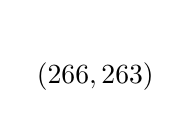
\begin{tikzpicture}[yscale=-1,every tree node/.style={draw, very thick, circle, inner sep=0.08cm}, level distance=0.7cm,sibling distance=0.3cm, , edge from parent path={[very thick, draw] (\tikzparentnode) -- (\tikzchildnode)}]]
	\Tree 
	[.\node{};
		[.\node{};
			[.\node{};]
		]
		[.\node{};]
		[.\node{};]
		[.\node{};]
	]
	\node(1) at (0,0.5) {$(266,263)$};
	\end{tikzpicture}}
	&
	\imagebot{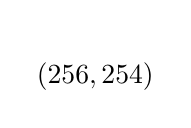
\begin{tikzpicture}[yscale=-1,every tree node/.style={draw, very thick, circle, inner sep=0.08cm}, level distance=0.7cm,sibling distance=0.3cm, , edge from parent path={[very thick, draw] (\tikzparentnode) -- (\tikzchildnode)}]]
	\Tree 
	[.\node{};
		[.\node{};]
		[.\node{};
			[.\node{};]
		]
		[.\node{};]
		[.\node{};]
	]
	\node(1) at (0,0.5) {$(256,254)$};
	\end{tikzpicture}}
	&
	\imagebot{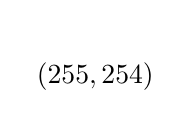
\begin{tikzpicture}[yscale=-1,every tree node/.style={draw, very thick, circle, inner sep=0.08cm}, level distance=0.7cm,sibling distance=0.3cm, , edge from parent path={[very thick, draw] (\tikzparentnode) -- (\tikzchildnode)}]]
	\Tree 
	[.\node{};
		[.\node{};]
		[.\node{};]
		[.\node{};
			[.\node{};]
		]
		[.\node{};]
	]
	\node(1) at (0,0.5) {$(255,254)$};
	\end{tikzpicture}}
	&
	\imagebot{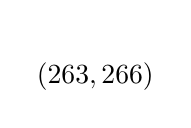
\begin{tikzpicture}[yscale=-1,every tree node/.style={draw, very thick, circle, inner sep=0.08cm}, level distance=0.7cm,sibling distance=0.3cm, , edge from parent path={[very thick, draw] (\tikzparentnode) -- (\tikzchildnode)}]]
	\Tree 
	[.\node{};
		[.\node{};]
		[.\node{};]
		[.\node{};]
		[.\node{};
			[.\node{};]
		]
	]
	\node(1) at (0,0.5) {$(263,266)$};
	\end{tikzpicture}}
	&
	\imagebot{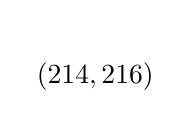
\begin{tikzpicture}[yscale=-1,every tree node/.style={draw, very thick, circle, inner sep=0.08cm}, level distance=0.7cm,sibling distance=0.3cm, , edge from parent path={[very thick, draw] (\tikzparentnode) -- (\tikzchildnode)}]]
	\Tree 
	[.\node{};
		[.\node{};
			[.\node{};]
				[.\node{};]
		]
		[.\node{};]
		[.\node{};]
	]
	\node(1) at (0,0.5) {$(214,216)$};
	\end{tikzpicture}}
	&
	\imagebot{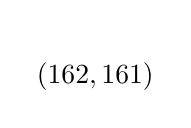
\begin{tikzpicture}[yscale=-1,every tree node/.style={draw, very thick, circle, inner sep=0.08cm}, level distance=0.7cm,sibling distance=0.3cm, , edge from parent path={[very thick, draw] (\tikzparentnode) -- (\tikzchildnode)}]]
	\Tree 
	[.\node{};
		[.\node{};
			[.\node{};]
		]
		[.\node{};
			[.\node{};]
		]
		[.\node{};]
	]
	\node(1) at (0,0.5) {$(162,161)$};
	\end{tikzpicture}}
	\\
	\imagebot{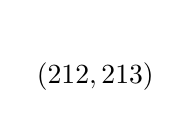
\begin{tikzpicture}[yscale=-1,every tree node/.style={draw, very thick, circle, inner sep=0.08cm}, level distance=0.7cm,sibling distance=0.3cm, , edge from parent path={[very thick, draw] (\tikzparentnode) -- (\tikzchildnode)}]]
	\Tree 
	[.\node{};
		[.\node{};]
		[.\node{};
			[.\node{};]
			[.\node{};]
		]
		[.\node{};]
	]
	\node(1) at (0,0.5) {$(212,213)$};
	\end{tikzpicture}}
	&	
	\imagebot{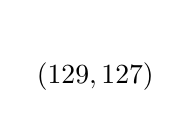
\begin{tikzpicture}[yscale=-1,every tree node/.style={draw, very thick, circle, inner sep=0.08cm}, level distance=0.7cm,sibling distance=0.3cm, , edge from parent path={[very thick, draw] (\tikzparentnode) -- (\tikzchildnode)}]]
	\Tree 
	[.\node{};
		[.\node{};]
		[.\node{};
			[.\node{};
				[.\node{};]
			]
		]
		[.\node{};]
	]
	\node(1) at (0,0.5) {$(129,127)$};
	\end{tikzpicture}}
		&
	\imagebot{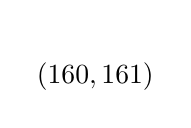
\begin{tikzpicture}[yscale=-1,every tree node/.style={draw, very thick, circle, inner sep=0.08cm}, level distance=0.7cm,sibling distance=0.3cm, , edge from parent path={[very thick, draw] (\tikzparentnode) -- (\tikzchildnode)}]]
	\Tree 
	[.\node{};
		[.\node{};]
		[.\node{};
			[.\node{};]
		]
		[.\node{};
			[.\node{};]
		]
	]
	\node(1) at (0,0.5) {$(160,161)$};
	\end{tikzpicture}}
	&
	\imagebot{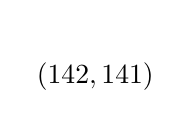
\begin{tikzpicture}[yscale=-1,every tree node/.style={draw, very thick, circle, inner sep=0.08cm}, level distance=0.7cm,sibling distance=0.3cm, , edge from parent path={[very thick, draw] (\tikzparentnode) -- (\tikzchildnode)}]]
	\Tree 
	[.\node{};
		[.\node{};  
			[.\node{};  
				[.\node{};]
			]
			[.\node{};] 
		]
		[.\node{};]
	]
	\node(1) at (0,0.5) {$(142,141)$};
	\end{tikzpicture}}
	&
	\imagebot{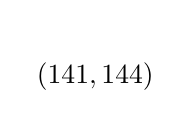
\begin{tikzpicture}[yscale=-1,every tree node/.style={draw, very thick, circle, inner sep=0.08cm}, level distance=0.7cm,sibling distance=0.3cm, , edge from parent path={[very thick, draw] (\tikzparentnode) -- (\tikzchildnode)}]]
	\Tree 
	[.\node{};
		[.\node{};  
			[.\node{};]
			[.\node{};] 
		]
		[.\node{};  
			[.\node{};] 
		]
	]
	\node(1) at (0,0.5) {$(141,144)$};
	\end{tikzpicture}}
	&
	\imagebot{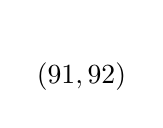
\begin{tikzpicture}[yscale=-1,every tree node/.style={draw, very thick, circle, inner sep=0.08cm}, level distance=0.7cm,sibling distance=0.3cm, , edge from parent path={[very thick, draw] (\tikzparentnode) -- (\tikzchildnode)}]]
	\Tree 
	[.\node{};
		[.\node{};  
			[.\node{};  
				[.\node{};] 
			]
		]
		[.\node{};  
			[.\node{};] 
		]
	]
	\node(1) at (0,0.5) {$(91,92)$};
	\end{tikzpicture}}
	\\
	\imagebot{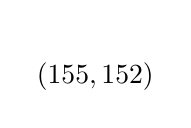
\begin{tikzpicture}[yscale=-1,every tree node/.style={draw, very thick, circle, inner sep=0.08cm}, level distance=0.7cm,sibling distance=0.3cm, , edge from parent path={[very thick, draw] (\tikzparentnode) -- (\tikzchildnode)}]]
	\Tree 
	[.\node{}; 
		[.\node{};  
			[.\node{};] 
		]
		[.\node{};  
			[.\node{};]
			[.\node{};] 
		]
	]
	\node(1) at (0,0.5) {$(155,152)$};
	\end{tikzpicture}}
		&
	\imagebot{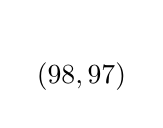
\begin{tikzpicture}[yscale=-1,every tree node/.style={draw, very thick, circle, inner sep=0.08cm}, level distance=0.7cm,sibling distance=0.3cm, , edge from parent path={[very thick, draw] (\tikzparentnode) -- (\tikzchildnode)}]]
	\Tree 
	[.\node{}; 
		[.\node{};  
			[.\node{};] 
		]
		[.\node{};  
			[.\node{};  
				[.\node{};] 
			]
		]
	]
	\node(1) at (0,0.5) {$(98,97)$};
	\end{tikzpicture}}
	&
	\imagebot{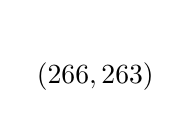
\begin{tikzpicture}[yscale=-1,every tree node/.style={draw, very thick, circle, inner sep=0.08cm}, level distance=0.7cm,sibling distance=0.3cm, , edge from parent path={[very thick, draw] (\tikzparentnode) -- (\tikzchildnode)}]]
	\Tree 
	[.\node{}; 
		[.\node{};]
		[.\node{};
			[.\node{};]
			[.\node{};]
			[.\node{};]
		]
	]
	\node(1) at (0,0.5) {$(266,263)$};
	\end{tikzpicture}}
	&  
	\imagebot{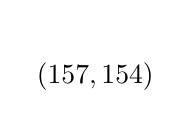
\begin{tikzpicture}[yscale=-1,every tree node/.style={draw, very thick, circle, inner sep=0.08cm}, level distance=0.7cm,sibling distance=0.3cm, , edge from parent path={[very thick, draw] (\tikzparentnode) -- (\tikzchildnode)}]]
	\Tree 
	[.\node{}; 
		[.\node{};]
		[.\node{};
			[.\node{};  
				[.\node{};] 
			]
			[.\node{};]
		]
	]
	\node(1) at (0,0.5) {$(157,154)$};
	\end{tikzpicture}}
	&
	\imagebot{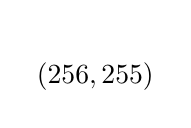
\begin{tikzpicture}[yscale=-1,every tree node/.style={draw, very thick, circle, inner sep=0.08cm}, level distance=0.7cm,sibling distance=0.3cm, , edge from parent path={[very thick, draw] (\tikzparentnode) -- (\tikzchildnode)}]]
	\Tree 
	[.\node{}; 
		[.\node{};
			[.\node{};
				[.\node{};]
			]
			[.\node{};]
			[.\node{};]
		]
	]
	\node(1) at (0,0.5) {$(256,255)$};
	\end{tikzpicture}}
	&
	\imagebot{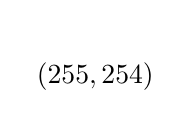
\begin{tikzpicture}[yscale=-1,every tree node/.style={draw, very thick, circle, inner sep=0.08cm}, level distance=0.7cm,sibling distance=0.3cm, , edge from parent path={[very thick, draw] (\tikzparentnode) -- (\tikzchildnode)}]]
	\Tree 
	[.\node{}; 
		[.\node{};
			[.\node{};]
			[.\node{};
				[.\node{};]
			]
			[.\node{};]
		]
	]
	\node(1) at (0,0.5) {$(255,254)$};
	\end{tikzpicture}}
	\\
	\imagebot{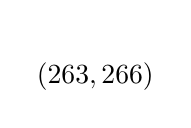
\begin{tikzpicture}[yscale=-1,every tree node/.style={draw, very thick, circle, inner sep=0.08cm}, level distance=0.7cm,sibling distance=0.3cm, , edge from parent path={[very thick, draw] (\tikzparentnode) -- (\tikzchildnode)}]]
	\Tree 
	[.\node{}; 
		[.\node{};
			[.\node{};]
			[.\node{};]
			[.\node{};
				[.\node{};]
			] 
		]
	]
	\node(1) at (0,0.5) {$(263,266)$};
	\end{tikzpicture}}
	&
	\imagebot{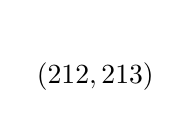
\begin{tikzpicture}[yscale=-1,every tree node/.style={draw, very thick, circle, inner sep=0.08cm}, level distance=0.7cm,sibling distance=0.3cm, , edge from parent path={[very thick, draw] (\tikzparentnode) -- (\tikzchildnode)}]]
	\Tree 
	[.\node{}; 
		[.\node{};
			[.\node{}; 
				[.\node{};]
				[.\node{};]
			] 
			[.\node{};]
		]
	]
	\node(1) at (0,0.5) {$(212,213)$};
	\end{tikzpicture}}  
	&
	\imagebot{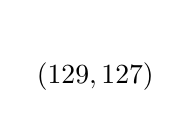
\begin{tikzpicture}[yscale=-1,every tree node/.style={draw, very thick, circle, inner sep=0.08cm}, level distance=0.7cm,sibling distance=0.3cm, , edge from parent path={[very thick, draw] (\tikzparentnode) -- (\tikzchildnode)}]]
	\Tree 
	[.\node{}; 
		[.\node{};
			[.\node{}; 
				[.\node{}; 
					[.\node{}; ]
				]
			] 
			[.\node{};]
		]
	]
	\node(1) at (0,0.5) {$(129,127)$};
	\end{tikzpicture}}
	&
	\imagebot{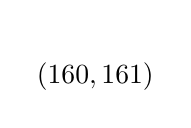
\begin{tikzpicture}[yscale=-1,every tree node/.style={draw, very thick, circle, inner sep=0.08cm}, level distance=0.7cm,sibling distance=0.3cm, , edge from parent path={[very thick, draw] (\tikzparentnode) -- (\tikzchildnode)}]]
	\Tree 
	[.\node{}; 
		[.\node{}; 
			[.\node{};  
				[.\node{};] 
			]
			[.\node{};  
				[.\node{};] 
			]
		]
	]
	\node(1) at (0,0.5) {$(160,161)$};
	\end{tikzpicture}}
	&
	\imagebot{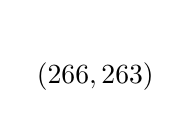
\begin{tikzpicture}[yscale=-1,every tree node/.style={draw, very thick, circle, inner sep=0.08cm}, level distance=0.7cm,sibling distance=0.3cm, , edge from parent path={[very thick, draw] (\tikzparentnode) -- (\tikzchildnode)}]]
	\Tree 
	[.\node{}; 
		[.\node{}; 
			[.\node{};
				[.\node{};]
				[.\node{};]
				[.\node{};] 
			]
		]
	]
	\node(1) at (0,0.5) {$(266,263)$};
	\end{tikzpicture}}
	&
	\imagebot{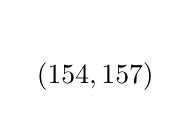
\begin{tikzpicture}[yscale=-1,every tree node/.style={draw, very thick, circle, inner sep=0.08cm}, level distance=0.7cm,sibling distance=0.3cm, , edge from parent path={[very thick, draw] (\tikzparentnode) -- (\tikzchildnode)}]]
	\Tree 
	[.\node{}; 
		[.\node{}; 
			[.\node{};
				[.\node{};  
					[.\node{};] 
				]
				[.\node{};]
			]
		]
	]
	\node(1) at (0,0.5) {$(154,157)$};
	\end{tikzpicture}}
\end{tabular}
\caption{The $24$ planar trees $t$ with $5$ internal edges for which the number of facets in the $\LA$ diagonal (left) and the $\SU$ diagonal (right) differ.}
\label{fig:trees}
\end{figure}

\begin{table}[h]
	\begin{center}
	\begin{tabular}{c|c|c|c|c|c} 
	Internal edges & $\LA$ diagonal & $\LA$ only & Shared & $\SU$ only & $\SU$ diagonal \\
	\hline
	$n=1$ & 2 & 0 & 2 & 0 & 2 \\
	$n=2$ & 8 & 0 & 8 & 0 & 8 \\
	$n=3$ & 42 & 5 & 37 & 5 & 42 \\
	$n=4$ & 254 & 72 & 182 & 72 & 254 \\
	$n=5$ & 1678 & 759 & 919 & 757 & 1676 \\
	$n=6$ & 11790 & 7076 & 4714 & 7024 & 11738 
	\end{tabular}
	\end{center}
	\caption{Number of facets in the $\LA$ and $\SU$ diagonals of the multiplihedra, indexed by linear trees with $n$ internal edges.}
	\label{table:multiplihedra}
\end{table}


